% ============================================================
% CHAPTER: Multi-Task Study -- Reconstruction, Captioning, and VQA
% Adapted from the QUEST conference submission draft.
% Follows the conventions established in Chapters 3-5:
% chapter summary inside \printmyminitoc, section-level intro
% paragraphs, an explicit Positioning subsection in Related Work.
% ============================================================
\titlespacing*{\chapter}{0pt}{-35pt}{40pt}
\chapter{A Multi-Task Study of Reconstruction, Captioning, and VQA}
\label{chap:multitask}
\startcontents[chapters]
\printmyminitoc{
\textit{Chapter summary.} The preceding chapters treated visual question answering as the sole training objective,
 whether on a single modality (Chapters~\ref{chap:llm_augmentation} and~\ref{chap:seg_attention}) or on the three co-registered modalities of TAMMI 
 (Chapter~\ref{chap:tammi}). This chapter instead studies what happens when RSVQA is trained jointly with captioning 
 and self-supervised image reconstruction, extending TAMMI with LLM-generated captions to support this joint setting. 
 This chapter compares four training configurations, full multi-task training, multi-task 
 training without reconstruction, VQA-only, and captioning-only, to measure the specific contribution of each additional 
 objective rather than the combination as a whole.
}
% ============================================================
\section{Introduction}
\label{sec:chap6_intro}

The previous two chapters extended RSVQA along two axes independently:
attention design (Chapter~\ref{chap:seg_attention}) and modality/resolution
coverage (Chapter~\ref{chap:tammi}). Both chapters, however, treated
RSVQA as the only training signal. Section~\ref{sec:rw-captioning-challenges}
already noted, in reviewing the RS literature, that models
combining RSVQA with other tasks (captioning in particular) are
increasingly common, but that the benefit of doing so is rarely measured
directly, and that where it has been measured, results are mixed rather
than confirmatory: RS-LLaVA's own reported results show single-task
fine-tuning outperforming joint training on both captioning and VQA
metrics, directly contradicting the premise behind combining the two
tasks. This chapter takes that open question as its object of study.

Remote sensing imagery is open to more than one training signal
beyond question answering. Captioning provides a free-form description
of a scene that is not constrained to a fixed answer vocabulary, and
self-supervised reconstruction provides a training signal that requires
no annotation at all, only the imagery itself. In principle, jointly
optimizing these three objectives, reconstruction, captioning, and VQA,
could encourage a shared representation that is more robust than any
one objective alone: reconstruction could preserve visual detail that a
purely discriminative VQA loss might discard, and captioning could
provide a richer, less templated supervisory signal than RSVQA's
templated question-answer pairs. Whether this potential is realized in
practice is what this
chapter investigates.

This chapter makes three contributions. First, we extend the TAMMI
dataset (Chapter~\ref{chap:tammi}) with LLM-generated captions,
producing a new RS benchmark supporting
reconstruction, captioning, and VQA jointly across the same
optical/multispectral/SAR triplets. Second, we introduce QUEST
(Questioning and Understanding Earth Observation Images
through Text), a unified
architecture that jointly optimizes global cross-modal contrastive
alignment, patch-level cross-modal alignment, per-modality
reconstruction, and a shared generative decoder for captioning and VQA,
so that all four objectives can be selectively enabled or disabled
within a single model rather than requiring separate architectures per
configuration. Third, rather than reporting a single best configuration,
we conduct a controlled study comparing four training configurations,
full multi-task training, multi-task training without reconstruction,
VQA-only, and captioning-only, isolating the contribution of
reconstruction and of joint training itself, respectively.

The remainder of this chapter is organized as follows.
Section~\ref{sec:chap6_related} reviews related work on multi-modal RS
datasets, RS vision-language models, self-supervised multi-modal RS
representation learning, and unified generative frameworks, and
positions this chapter's ablation-based study relative to each.
Section~\ref{sec:chap6_dataset} describes the caption extension of
TAMMI. Section~\ref{sec:chap6_method} presents the architecture and
training objectives. Section~\ref{sec:chap6_experiments} reports and
discusses the results of the four-configuration study.
Section~\ref{sec:chap6_conclusion} concludes and discusses limitations.

\section{Related Work}
\label{sec:chap6_related}

This section reviews four bodies of work relevant to this chapter's
study. Section~\ref{sec:chap6_rw_datasets} reviews multi-modal RS
datasets.
Section~\ref{sec:chap6_rw_vlm} reviews RS vision-language models that, combine multiple language-producing tasks, but
without isolating each task's contribution. Section~\ref{sec:chap6_rw_ssl}
reviews self-supervised multi-modal RS representation learning, which
grounds cross-modal alignment without language. Section~\ref{sec:chap6_rw_unified}
reviews unified generative frameworks outside RS. Section~\ref{sec:chap6_positioning}
then positions this chapter's contribution relative to all four.

\subsection{Multi-Modal Remote Sensing Datasets}
\label{sec:chap6_rw_datasets}

The availability of large-scale, annotated multi-modal datasets has
been a key driver of progress in Earth observation.
\textcite{schmitt2019sen12mscurateddataset} established an early benchmark with
SEN12MS, providing 180,662 co-registered Sentinel-1 SAR and Sentinel-2
multispectral image triplets paired with MODIS land cover maps, enabling
data fusion research at scale. \textcite{sumbul2019bigearthnet} extended
this effort with BigEarthNet, 590,326 Sentinel-2 patches annotated with
multi-label CORINE land cover classes, later expanded to include paired
Sentinel-1 imagery. More recently, BigEarthNet.txt~\cite{herzog2026bigearthnettxt}
enriched the BigEarthNet corpus with around 9.6 million text
annotations, including geographically anchored captions, VQA pairs, and
referring expression instructions over co-registered Sentinel-1/2
pairs, and ChatEarthNet~\cite{yuan2024chatearth} provides 163K
Sentinel-2 image-caption pairs generated using a general-purpose LLM,
covering global land cover types. Despite this progress, none of these
datasets incorporate VHR RGB imagery alongside SAR and multispectral
data at the resolution TAMMI does; conversely, TAMMI itself
(Chapter~\ref{chap:tammi}) supports VQA but not free-form captioning.
%This chapter extends TAMMI with LLM-generated captions to close that
%gap, discussed in full in Section~\ref{sec:chap6_dataset}.

\subsection{Vision-Language Models for Remote Sensing}
\label{sec:chap6_rw_vlm}

Early vision-language work in RS focused on adapting contrastive
image-text pretraining to the domain. RemoteCLIP~\cite{liu2024remoteclip}
was the first vision-language foundation model tailored to RS, training
a CLIP-style model on a scaled dataset built by converting heterogeneous
annotations into image-caption pairs. RS-M-CLIP~\cite{silva2024rsmclip}
extended this to multilingual settings, showing that aligning local and
global representations improves cross-modal retrieval. These contrastive
models are effective for retrieval and zero-shot classification but do
not support generative tasks such as captioning or VQA.

Instruction-tuned VLMs have since expanded the scope of language-driven
RS analysis. GeoChat~\cite{kuckreja2024geochat} was the first grounded
VLM for RS, fine-tuning LLaVA-1.5 on a curated RS instruction dataset to
support image and region captioning, VQA, scene classification, and
referring object detection on high-resolution RGB imagery. EarthDial~\cite{soni2025earthdialturningmultisensoryearth}
scales this paradigm further, fine-tuning InternVL on an
instruction dataset spanning RGB, multispectral, SAR, and multi-temporal
data, and SkyEyeGPT~\cite{zhan2025skyeyegpt} similarly unifies multiple
RS vision-language tasks via instruction tuning. All of these approaches
adapt a pretrained LLM through projection layers without explicitly
enforcing cross-modal spatial alignment: the model has no mechanism to
associate co-registered patches from different sensors in the embedding
space beyond what is implicitly learned through language supervision.
%None of these works
%isolates the contribution of the individual tasks their instruction
%data combines.

\subsection{Multi-Modal Representation Learning in Earth Observation}
\label{sec:chap6_rw_ssl}

A parallel line of work learns grounded multi-modal representations
through self-supervised objectives, without language.
DINO-MM~\cite{scheibenreif2022dinomm} applies a DINO-style
self-supervised framework jointly to Sentinel-1 and Sentinel-2 pairs,
learning complementary SAR-optical representations via intra- and
inter-modality objectives. CROMA~\cite{fuller2023croma} combines
cross-modal contrastive learning with masked autoencoding over
co-registered SAR and multispectral samples, showing that these
objectives are complementary on spatially aligned data.
Fus-MAE~\cite{chanthonghong2024fusmae} proposes a cross-attention-based
masked autoencoder for early and feature-level SAR-optical fusion,
competitive with contrastive approaches while requiring no augmentation
design. These methods demonstrate the value of explicit cross-modal
alignment for representation quality, but they are entirely visual:
language is absent, and the learned representations cannot be directly
applied to captioning or VQA. 

\subsection{Unified Generative Frameworks for Vision and Language}
\label{sec:chap6_rw_unified}

Outside of Remote Sensing, unified encoder-decoder architectures such as
VL-T5~\cite{cho2021vlt5} demonstrated that a single sequence-to-sequence
model can handle both captioning and VQA by casting all tasks as text
generation. This design principle, a single shared decoder across
tasks rather than task-specific decoding heads, motivates this
chapter's use of a shared FLAN-T5 decoder~\cite{chung2022flant5} for
both captioning and VQA, enabling the two tasks to share generative
capacity and, in principle, transfer between each other, the specific
question this chapter's study addresses.

\subsection{Positioning}
\label{sec:chap6_positioning}

The datasets and architectures reviewed above are each necessary but not
individually sufficient for this chapter's study. TAMMI provides the
three-modality imagery this chapter builds on but no captions;
BigEarthNet.txt and ChatEarthNet provide captions but not VHR imagery
paired with SAR and multispectral data at TAMMI's resolution. RS
vision-language models already train on combined caption and VQA data,
but, as discussed in Section~\ref{sec:chap6_rw_vlm}, do not isolate
what each task contributes, and a directly comparable measurement
available (RS-LLaVA) found joint training to underperform single-task
training. Self-supervised multi-modal RS representation learning
demonstrates that explicit cross-modal grounding improves
representation quality, but without a language interface to evaluate
that improvement on captioning or VQA directly. This chapter combines cross-modal
grounding and a shared generative decoder, specifically to run the
controlled comparison: whether reconstruction and joint captioning-VQA
training measurably help, rather than assuming they do.

\section{Extending TAMMI with Captions}
\label{sec:chap6_dataset}

This chapter reuses the TAMMI dataset introduced in
Chapter~\ref{chap:tammi}: VHR optical, Sentinel-2 multispectral, and
Sentinel-1 SAR triplets with RSVQA question-answer pairs across six
departments of Metropolitan France. We extend it with free-form
captions, used here for the captioning.

Captions are generated in two stages. First, a \textit{raw caption} is
constructed automatically. Each VHR patch is divided into a
$3\times3$ spatial grid (top-left, top-center, \ldots, bottom-right).
For each cell, we enumerate the BD TOPO object classes present and
their approximate location. We use 24 BD TOPO feature classes,
covering buildings, cemeteries, linear/point/surface constructions,
pylons, reservoirs, sports fields, hydrographic features, vegetation
zones, pipelines, power infrastructure, activity zones, aerodromes,
and transport infrastructure (road, rail, cable). Classes are
translated from French BD TOPO nomenclature to English via a
class- and nature-specific mapping. This 24-class list is a superset
of both the 16-class segmentation taxonomy of
Chapter~\ref{chap:seg_attention} and TAMMI's own question-generation
taxonomy (Chapter~\ref{chap:tammi}). Repeated mentions of the same
class within a cell are merged into a single count, e.g. "three
buildings" rather than three separate mentions. The result is a
structured but non-fluent list of (class, location, count) triplets.

Second, an LLM reformulates the raw caption into a single fluent
English sentence. We use Gemma 3 (27B parameters). The LLM may rephrase and combine the given facts, but may not
invent new information. It must describe objects naturally rather
than by their raw class labels (e.g. not "hedge4" or "motorway
type1"), and must not produce a numbered list. 

Captions follow the same train/validation/test split as TAMMI's
question-answer pairs (Chapter~\ref{chap:tammi},
Section~\ref{sec:chap5_splitting}): no caption and its corresponding
VQA pairs fall in different partitions. In total, 271,416 captions
were generated across all six of TAMMI's departments (75, 92, 93, 94,
74, 34): 162,459 for training, 54,194 for validation, and 54,763 for
testing.

\section{The QUEST Architecture}
\label{sec:chap6_method}

This section presents QUEST in five parts.
Section~\ref{sec:chap6_method_overview} gives a high-level overview.
Section~\ref{sec:chap6_method_encoders} describes the modality-specific
visual encoders. Section~\ref{sec:chap6_method_fusion} describes text
encoding and multi-modal fusion. Section~\ref{sec:chap6_method_contrastive}
presents the cross-modal contrastive objectives, and
Section~\ref{sec:chap6_method_reconstruction} the reconstruction
objective. Section~\ref{sec:chap6_method_decoding} describes the shared
captioning/VQA decoder, and Section~\ref{sec:chap6_method_loss} the
combined training objective that the study in
Section~\ref{sec:chap6_experiments} selectively ablates.

\subsection{Overview}
\label{sec:chap6_method_overview}

QUEST jointly models three heterogeneous
Earth observation modalities, VHR RGB, Sentinel-1 SAR, and Sentinel-2
multispectral imagery, together with natural-language inputs such as
captions and VQA queries. The goal is a shared latent space that is
simultaneously semantically aligned across modalities, spatially
grounded, and expressive enough to support both generative and
discriminative tasks. Unlike prior work that either aligns a single
optical modality with text or jointly models multiple RS modalities
without language (Section~\ref{sec:chap6_related}), QUEST
unifies three heterogeneous satellite modalities and natural language
within a single generative and contrastive framework, combining a
fixed-token multi-resolution design that preserves spatial
correspondences across resolutions, global and patch-level cross-modal
alignment losses, and a shared language decoder for both captioning and
VQA.

Let $x = (x^{\text{VHR}}, x^{\text{S2}}, x^{\text{S1}}, t)$ denote a
training sample, where $t$ is a text input (a caption or a VQA
question). All modalities are mapped into a shared $d = 256$
dimensional embedding space and processed jointly through a fusion
transformer that produces a unified representation used for downstream
tasks. Figure~\ref{fig:chap6_architecture} gives an overview of the
full pipeline, detailed section by section in the remainder of this
section.

\begin{figure}[ht]
\centering
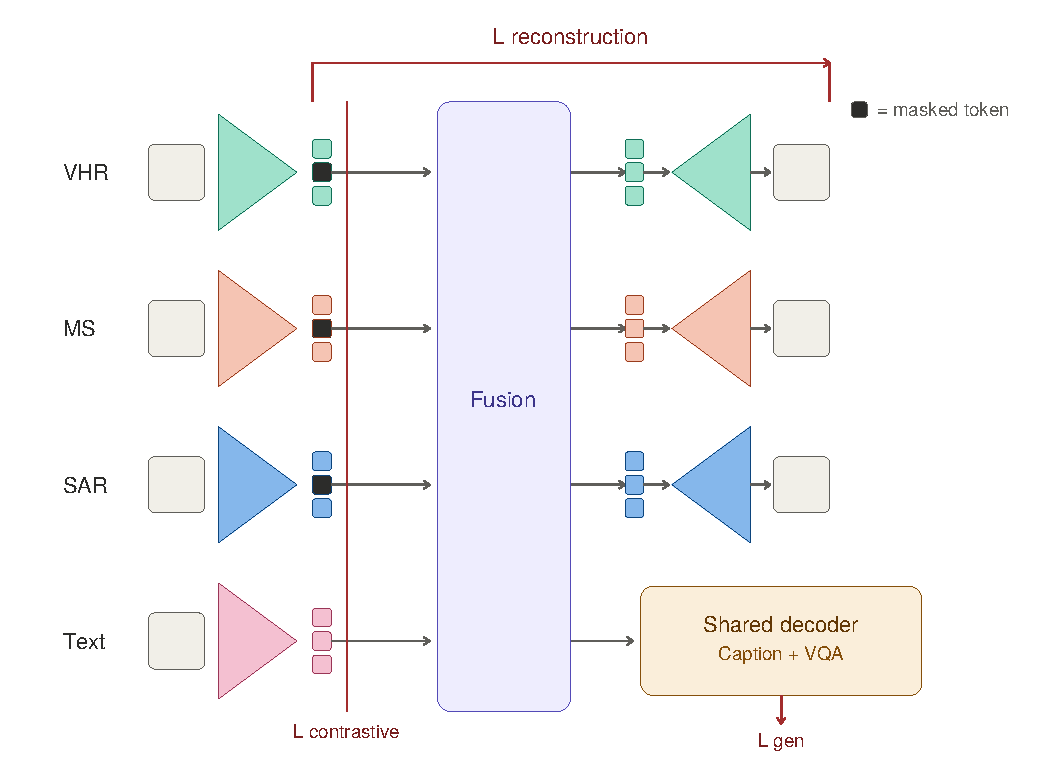
\includegraphics[width=0.95\textwidth]{images/multitask/quest_architecture_v2.pdf}
\caption{Overview of the QUEST architecture. Each modality is encoded
into patch tokens, a subset of which are masked (black squares) before
fusion, following the masked-patch-prediction strategy of
\textcite{astruc2024omnisat}. The fused representation feeds three
objectives: $\mathcal{L}_\text{reconstruction}$ predicts the masked
tokens' original content per visual modality,
$\mathcal{L}_\text{contrastive}$ aligns unmasked token embeddings
across all four modalities, and $\mathcal{L}_\text{gen}$ supervises
the shared captioning/VQA decoder. Only the objectives active in a
given configuration (Table~\ref{tab:chap6_configs}) are used during
training.}
\label{fig:chap6_architecture}
\end{figure}

\subsection{Multi-Modal Visual Encoders}
\label{sec:chap6_method_encoders}

Although the three visual modalities differ in spatial resolution,
spectral structure, and sensing physics, modality-specific encoders
convert each input into a sequence of $N = 100$ latent tokens in the
shared embedding space. This token count is the largest supported by
each modality's native resolution without upsampling (VHR
$1000\times1000$, SAR $200\times200$, multispectral $100\times100$),
balancing meaningful spatial footprint per token against fusion
compute.

\textbf{VHR RGB.} High-resolution RGB images are divided into
non-overlapping $100\times100$ patches. Each patch is flattened and
passed through a linear projection layer into the shared embedding
dimension, producing tokens $\{z^{\text{VHR}}_i\}_{i=1}^{N}$.

\textbf{Sentinel-2 multispectral.} Sentinel-2 inputs contain ten
spectral bands at heterogeneous native resolutions. A lightweight
convolutional stem (strided convolutions, pooling, and residual
blocks) harmonizes these bands and captures spectral interactions; the
resulting feature map is partitioned into $10\times10$ patches, each
projected into the shared embedding space to obtain tokens
$\{z^{\text{S2}}_i\}_{i=1}^{N}$.

\textbf{Sentinel-1 SAR.} SAR images are divided into $20\times20$
patches and passed through a linear projection layer, yielding tokens
$\{z^{\text{S1}}_i\}_{i=1}^{N}$.

\textbf{Shared transformer encoder.} For each modality
$m \in \{\text{VHR}, \text{S2}, \text{S1}\}$, a learnable class token
is prepended and modality-specific positional embeddings are added.
The resulting sequence is processed by a 6-layer transformer encoder
with 16 attention heads and an MLP expansion ratio of 4, producing
modality-aware latent representations
\[
\tilde{Z}^{m} = \text{TransformerEnc}(Z^{m}),
\]
which serve as the visual inputs to the fusion module.

\subsection{Text Encoder and Multi-Modal Fusion}
\label{sec:chap6_method_fusion}

Text inputs (captions or VQA queries) are encoded using a pretrained
T5 encoder. The resulting token embeddings are projected into the
shared $d = 256$ dimensional space and concatenated with the visual
tokens from all available modalities. The combined sequence is
processed by a transformer-based fusion module that uses self-attention
to integrate high-resolution spatial cues, multispectral information,
SAR patterns, and linguistic semantics. The output of this module,
denoted $F$, forms a unified representation supporting both contrastive
learning and generative decoding.

\subsection{Cross-Modal Contrastive Learning}
\label{sec:chap6_method_contrastive}

To enforce semantic consistency across modalities, two contrastive
objectives are used.

\textbf{Global image-text alignment.} For each visual modality $m$, a
pooled embedding is obtained by mean-pooling over its patch tokens,
denoted $g^{m}$, and a pooled text embedding $g^{\text{text}}$ is
obtained by mean-pooling over the caption tokens. A separate InfoNCE
term is computed per modality and summed, bringing matched image-text
pairs closer while pushing mismatched pairs apart, with a learned
temperature $\tau$:
\[
\mathcal{L}_{\text{global}} = \sum_{m} \left[ -\frac{1}{B} \sum_{i=1}^{B}
\log \frac{\exp(\text{sim}(g^{m}_i, g^{\text{text}}_i)/\tau)}
{\sum_{j=1}^{B} \exp(\text{sim}(g^{m}_i, g^{\text{text}}_j)/\tau)} \right].
\]
 
\textbf{Cross-modal visual alignment.} When resolutions differ,
correspondences are defined in the normalized spatial coordinate
system of the image: each patch token is associated with the center
coordinates of its receptive field, normalized to $[0,1]^2$. For two
modalities $m_1 \neq m_2$, each patch of $m_1$ is matched to the
geographically closest patch center of $m_2$, yielding a one-to-one or
one-to-many correspondence depending on resolution, without requiring
external registration beyond the co-registered imagery already
provided by TAMMI. The loss is
\[
\mathcal{L}_{\text{local-vis}} = -\frac{1}{B} \sum_{i}
\log \frac{\exp(\text{sim}(z^{m_1}_i, z^{m_2}_i)/\tau)}
{\sum_{k} \exp(\text{sim}(z^{m_1}_i, z^{m_2}_k)/\tau)}.
\]

\subsection{Visual Reconstruction}
\label{sec:chap6_method_reconstruction}

To prevent the shared representation from collapsing to purely
semantic features, each visual modality is equipped with a
reconstruction head trained via masked patch prediction. Concretely,
tokens across the three visual modalities are masked jointly, before
text tokens are concatenated, so that text is never masked and always
provides an unmasked conditioning signal: for each sample, a random
subset of visual token positions is selected via per-sample shuffling
(sorting random noise and keeping the first $\lfloor L(1-r)\rfloor$
positions, where $L$ is the total number of visual tokens and $r =
0.5$ is the masking ratio), and each masked position is replaced by a
shared, learned mask token rather than being removed from the
sequence or zeroed out.
The corresponding decoder $D_m$ is then trained to predict the
original patch content $\hat{x}^{m}_i$ for the masked tokens from the
fused representation, supervised with an $\ell_2$ loss:
\[
\mathcal{L}_{\text{rec}} = \sum_{m} \sum_{i \in \mathcal{M}^m}
\| \hat{x}^{m}_i - x^{m}_i \|_2^2,
\]
where $\mathcal{M}^m$ denotes the set of masked token indices for
modality $m$. Masking, rather than reconstructing every token
unconditionally, forces the decoder to rely on cross-modal and
spatial context propagated through the fusion module rather than
trivially copying each token's own visual encoding forward. For
modalities undergoing learned downsampling (Sentinel-2), the decoder
uses pooling indices from the encoder to restore spatial structure.
This is the objective ablated in
Section~\ref{sec:chap6_experiments} between the "w/ reco" and "w/o
reco" configurations.

\subsection{Captioning and Visual Question Answering}
\label{sec:chap6_method_decoding}

The fused representation $F$ is projected to the T5 hidden dimension
and used as encoder-side context for a T5 autoregressive decoder. The
decoder attends jointly to all visual and textual tokens via
cross-attention and generates either a caption or a VQA answer. A
single decoder is shared across both tasks, so that any transfer
between captioning and VQA is a property of the shared decoder rather
than of two independently trained heads, matching the study's goal of
measuring whether such transfer occurs rather than assuming it by
architectural construction.

\subsection{Total Loss}
\label{sec:chap6_method_loss}

The full training objective combines all components:
\[
\mathcal{L} = \lambda_{\text{global}} \mathcal{L}_{\text{global}}
+ \lambda_{\text{local-vis}} \mathcal{L}_{\text{local-vis}}
+ \lambda_{\text{rec}} \mathcal{L}_{\text{rec}}
+ \lambda_{\text{gen}} \mathcal{L}_{\text{gen}},
\]
where $\mathcal{L}_{\text{gen}}$ is the standard autoregressive
cross-entropy loss for captioning and VQA. Each of
$\lambda_{\text{rec}}$, and the presence of captioning versus VQA data
in $\mathcal{L}_{\text{gen}}$, is set to zero for the corresponding
ablated configuration in the study that follows, rather than requiring
separately trained architectures per configuration.

\section{Experimental Study}
\label{sec:chap6_experiments}

This section reports the four-configuration study motivated in
Section~\ref{sec:chap6_intro}. Section~\ref{sec:chap6_setup} defines
the four configurations and the evaluation protocol.
Section~\ref{sec:chap6_results} reports captioning and VQA metrics
across all four. Section~\ref{sec:chap6_results} examines individual examples in detail. Section~\ref{sec:chap6_discussion} discusses
these results, what they establish about the value of joint
training.

\subsection{Experimental Setup}
\label{sec:chap6_setup}

Four training configurations are compared, each obtained by enabling
or disabling terms of $\mathcal{L}$ (Section~\ref{sec:chap6_method_loss})
rather than by training separate architectures:

\begin{itemize}
\item \textbf{w/ reco}: the full model, trained with reconstruction,
contrastive alignment, captioning, and VQA jointly.
\item \textbf{w/o reco}: identical to \textbf{w/ reco} but with
$\lambda_{\text{rec}} = 0$, isolating the contribution of the
reconstruction objective specifically.
\item \textbf{VQA only}: $\mathcal{L}_{\text{gen}}$ restricted to VQA
and $\lambda_{\text{rec}} = 0$, with $\mathcal{L}_{\text{global}}$ and
$\mathcal{L}_{\text{local-vis}}$ still active; the single-task
baseline for VQA with respect to the generative and reconstruction
objectives specifically, though not a purely single-objective model.
\item \textbf{Caption only}: $\mathcal{L}_{\text{gen}}$ restricted to
captioning and $\lambda_{\text{rec}} = 0$, with $\mathcal{L}_{\text{global}}$
and $\mathcal{L}_{\text{local-vis}}$ still active; the single-task
baseline for captioning with respect to the generative and
reconstruction objectives specifically, though not a purely
single-objective model.
\end{itemize}

Table~\ref{tab:chap6_configs} summarizes which terms of
$\mathcal{L}$ are active in each configuration.

\begin{table}[ht]
\centering
\small
\caption{Loss terms active in each of the four training
configurations compared in this study. $\mathcal{L}_\text{global}$ and
$\mathcal{L}_\text{local-vis}$ are active in every configuration; only
$\mathcal{L}_\text{rec}$ and the task restriction on $\mathcal{L}_\text{gen}$
are ablated.}
\label{tab:chap6_configs}
\begin{tabular}{lccccc}
\toprule
\textbf{Configuration} & $\mathcal{L}_{\text{global}}$ & $\mathcal{L}_{\text{local-vis}}$ & $\mathcal{L}_{\text{rec}}$ & $\mathcal{L}_{\text{gen}}$ (caption) & $\mathcal{L}_{\text{gen}}$ (VQA) \\
\midrule
w/ reco       & \checkmark & \checkmark & \checkmark & \checkmark & \checkmark \\
w/o reco      & \checkmark & \checkmark &            & \checkmark & \checkmark \\
VQA only      & \checkmark & \checkmark &            &            & \checkmark \\
Caption only  & \checkmark & \checkmark &            & \checkmark &            \\
\bottomrule
\end{tabular}
\end{table}
All four configurations are trained on the same TAMMI splits
(Chapter~\ref{chap:tammi}, Section~\ref{sec:chap5_splitting}), extended
with the captions described in Section~\ref{sec:chap6_dataset}. All
models are optimized with Adam~\cite{kingma2015adam} at a learning
rate of $10^{-6}$ (no weight decay), with a
plateau-based learning rate decay scheduler (factor 0.1, patience 10 epochs)
monitoring validation loss, trained for a minimum of 14 and a maximum
of 20 epochs, and a batch
size of 16 per step. For the non-ablated terms of $\mathcal{L}$
(Section~\ref{sec:chap6_method_loss}), $\lambda_\text{rec} = 1.0$,
$\lambda_\text{local-vis} = 0.04$, and $\lambda_\text{global} = 0.18$.
Captioning is evaluated with ROUGE-1 and ROUGE-L, and with BERTScore
computed at four similarity thresholds (60, 70, 80, 90) to assess how
performance degrades as the required similarity to the reference
caption becomes stricter. VQA is evaluated with overall accuracy and with the
same BERTScore-threshold protocol applied to the generated answer text.
\subsection{Quantitative Results}
\label{sec:chap6_results}

Table~\ref{tab:chap6_captioning} reports captioning metrics and
Table~\ref{tab:chap6_vqa} reports VQA metrics across all four
configurations.

\begin{table}[ht]
\centering
\small
\caption{Captioning results across the four training configurations.
ROUGE scores are reported directly; BERTScore is reported as the
fraction of generated captions exceeding each similarity threshold.}
\label{tab:chap6_captioning}
\begin{tabular}{lcccc}
\toprule
\textbf{Metric} & \textbf{w/ reco} & \textbf{w/o reco} & \textbf{VQA only} & \textbf{Caption only} \\
\midrule
ROUGE-1 & 0.5055 & \textbf{0.5159} & -- & 0.5032 \\
ROUGE-L & 0.4173 & \textbf{0.4227} & -- & 0.4183 \\
BERTScore @ 60 & 1.0000 & 1.0000 & -- & 1.0000 \\
BERTScore @ 70 & 0.9997 & \textbf{1.0000} & -- & \textbf{1.0000} \\
BERTScore @ 80 & 0.9871 & \textbf{0.9891} & -- & 0.9873 \\
BERTScore @ 90 & 0.2288 & 0.2344 & -- & \textbf{0.2355} \\
\bottomrule
\end{tabular}
\end{table}

\begin{table}[ht]
\centering
\small
\caption{VQA results across the four training configurations.
BERTScore is reported as the fraction of generated answers exceeding
each similarity threshold.}
\label{tab:chap6_vqa}
\begin{tabular}{lcccc}
\toprule
\textbf{Metric} & \textbf{w/ reco} & \textbf{w/o reco} & \textbf{VQA only} & \textbf{Caption only} \\
\midrule
Overall Accuracy & 0.5613 & 0.5619 & \textbf{0.5769} & -- \\
BERTScore @ 60 & 0.9987 & 0.9982 & \textbf{0.9999} & -- \\
BERTScore @ 70 & 0.9525 & \textbf{0.9555} & 0.9550 & -- \\
BERTScore @ 80 & 0.8572 & 0.8558 & \textbf{0.8644} & -- \\
BERTScore @ 90 & 0.7571 & 0.7470 & \textbf{0.7589} & -- \\
\bottomrule
\end{tabular}
\end{table}

On captioning, w/o reco slightly outperforms w/ reco on both ROUGE
metrics (0.5159 vs.\ 0.5055 ROUGE-1; 0.4227 vs.\ 0.4173 ROUGE-L) and
tracks close to the Caption-only single-task baseline across all six
metrics, with no metric where w/ reco is the best of the three. On
VQA, VQA-only outperforms both multi-task configurations on every
metric, most notably on overall accuracy (0.5769 vs.\ 0.5613--0.5619).
Neither task, at the level of these aggregate metrics, shows joint
training outperforming its corresponding single-task baseline.

\subsection{Qualitative Analysis}
\label{sec:chap6_qualitative}

Aggregate metrics average over all question types and caption content
uniformly, which can mask effects specific to a particular question
type or scene. This section examines four individual examples, each
selected to test a specific aspect of the quantitative results above:
a failure shared across all configurations, a case where joint
training succeeds despite losing on aggregate, a captioning comparison
that stress-tests what BERTScore actually rewards, and the
reconstruction quality underlying $\mathcal{L}_\text{rec}$ itself.

\begin{figure}[ht]
\centering
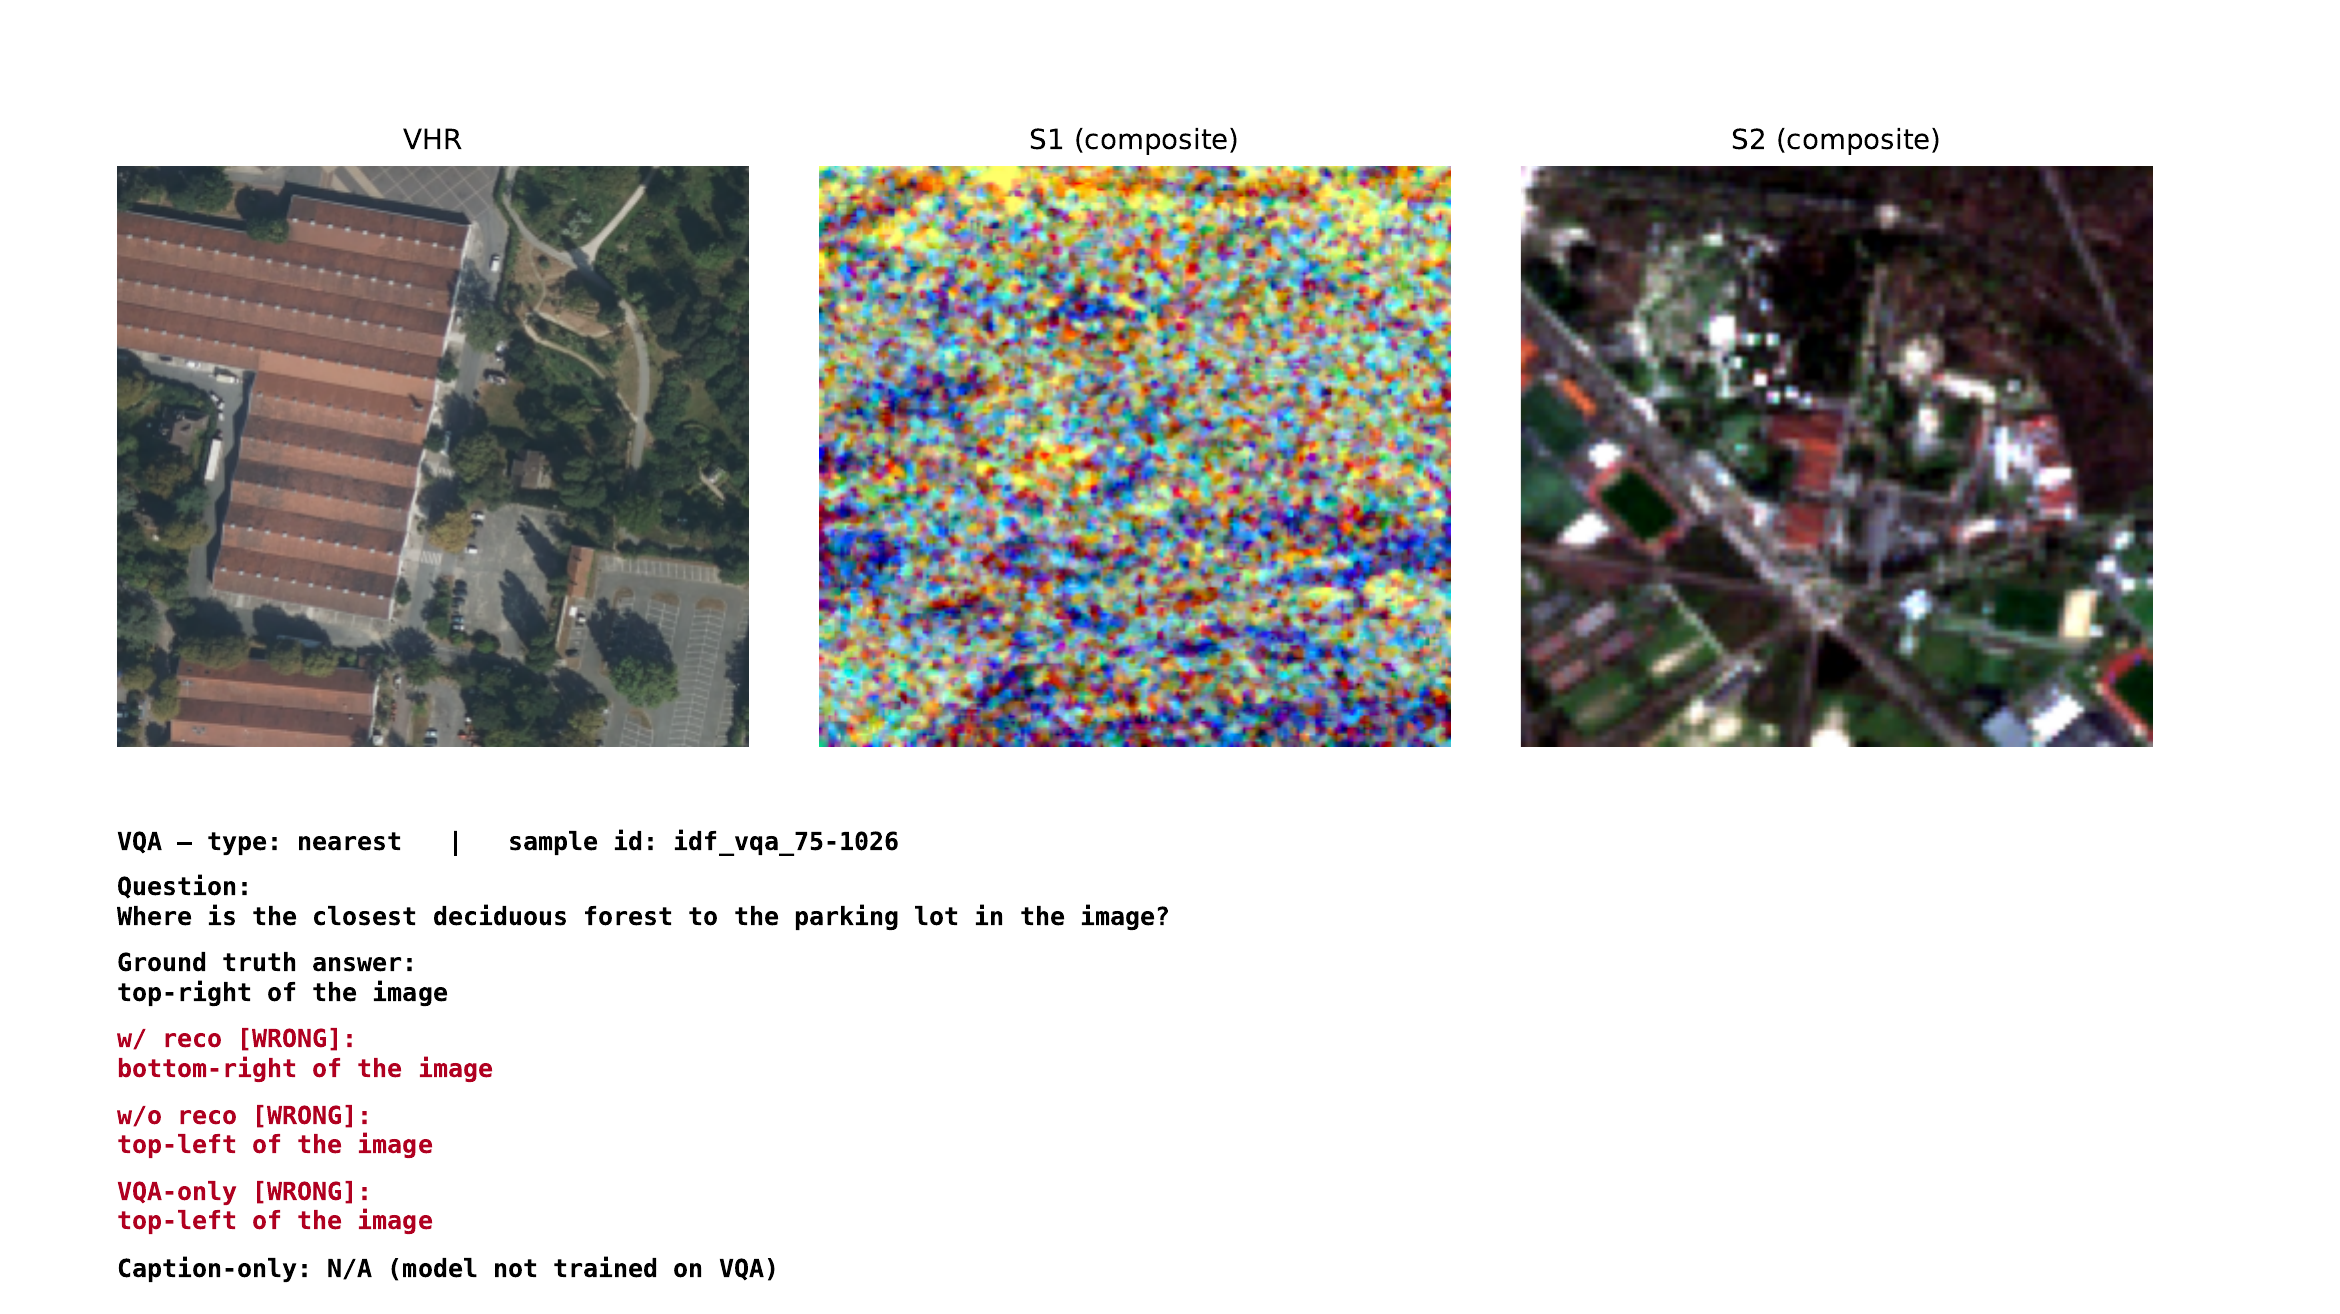
\includegraphics[width=0.85\textwidth]{images/multitask/qual_vqa_failure.png}
\caption{A \textit{nearest} question
on which all configurations answer incorrectly, converging on
different but equally wrong directions.}
\label{fig:chap6_qual_vqa_fail}
\end{figure}

In Figure~\ref{fig:chap6_qual_vqa_fail}, all configurations answer this \textit{nearest} question
incorrectly, each converging on a different wrong direction rather
than a shared one. This is consistent with two compounding
difficulties rather than a single cause: ambiguity in what "nearest"
refers to when several candidate objects are plausible, and the
resolution limits on resolving fine spatial relations discussed
throughout this thesis. Since the failure is shared across every
configuration, including VQA-only, it is not attributable to
multi-task training specifically, and is better read as a property of
the question type itself.

\begin{figure}[ht]
\centering
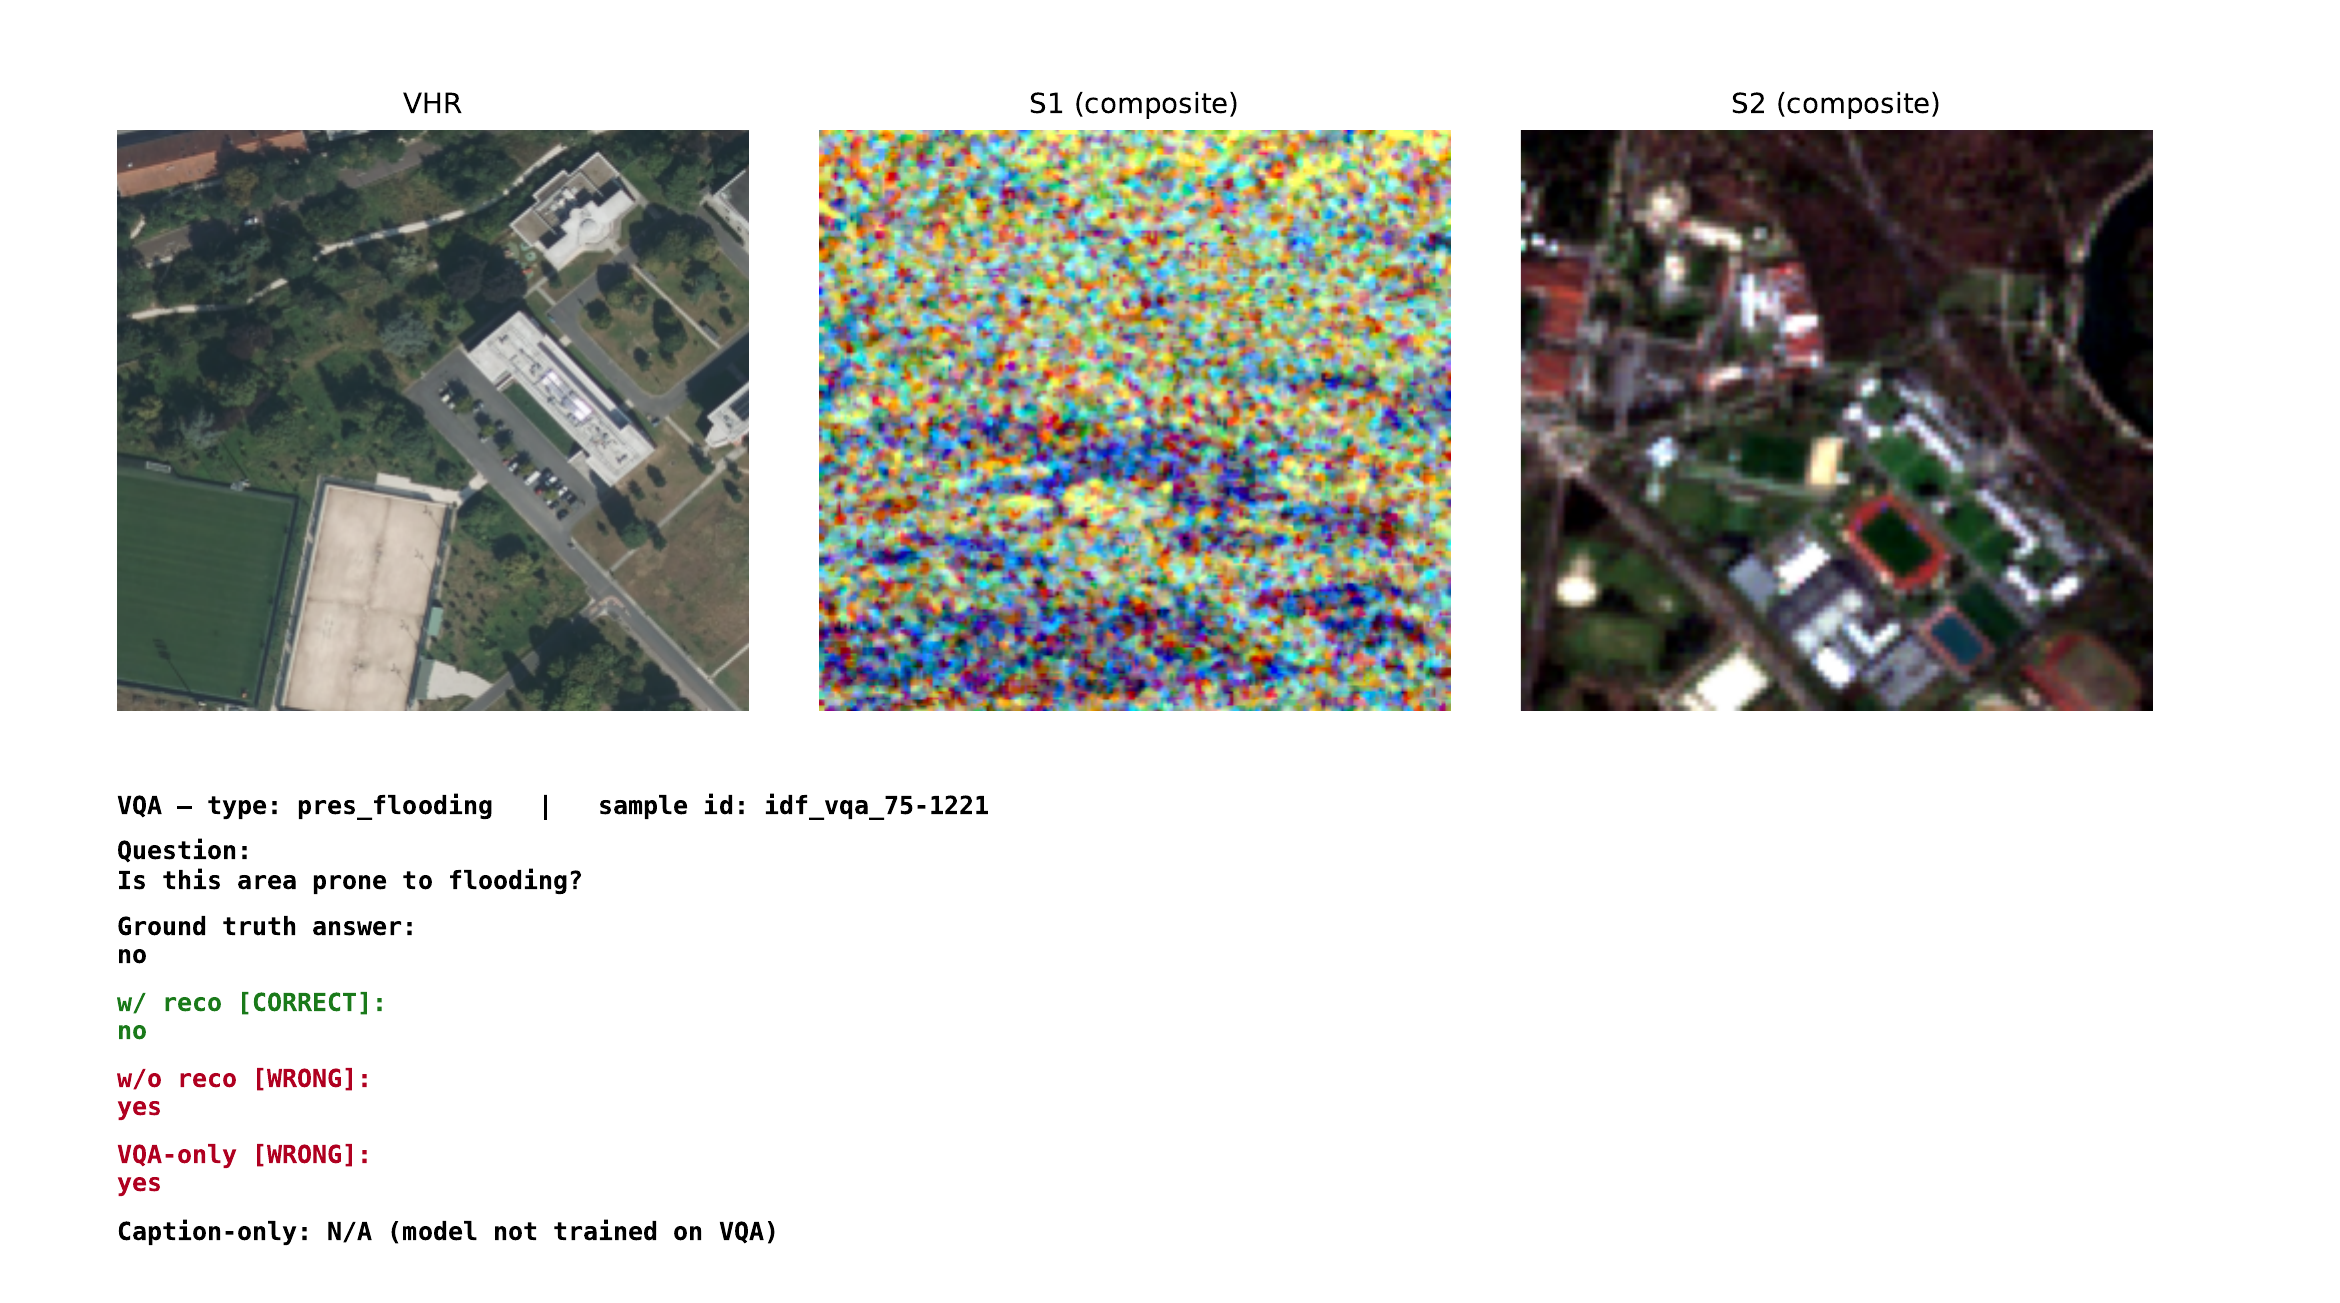
\includegraphics[width=0.85\textwidth]{images/multitask/qual_vqa_success.png}
\caption{A \textit{Flooding Presence} question on which the full multi-task model (w/
reco) answers correctly while both w/o reco and VQA-only answer
incorrectly.}
\label{fig:chap6_qual_vqa_success}
\end{figure}

The example in Figure~\ref{fig:chap6_qual_vqa_success} is a direct counter-example to the aggregate accuracy
result in Table~\ref{tab:chap6_vqa}: although VQA-only wins on
average, here it is the full multi-task model that answers correctly
while the single-task baseline does not. A single example cannot
establish how common this pattern is, but it demonstrates that the
aggregate result is compatible with joint training helping on specific
question types, rather than ruling this out.

\begin{figure}[ht]
\centering
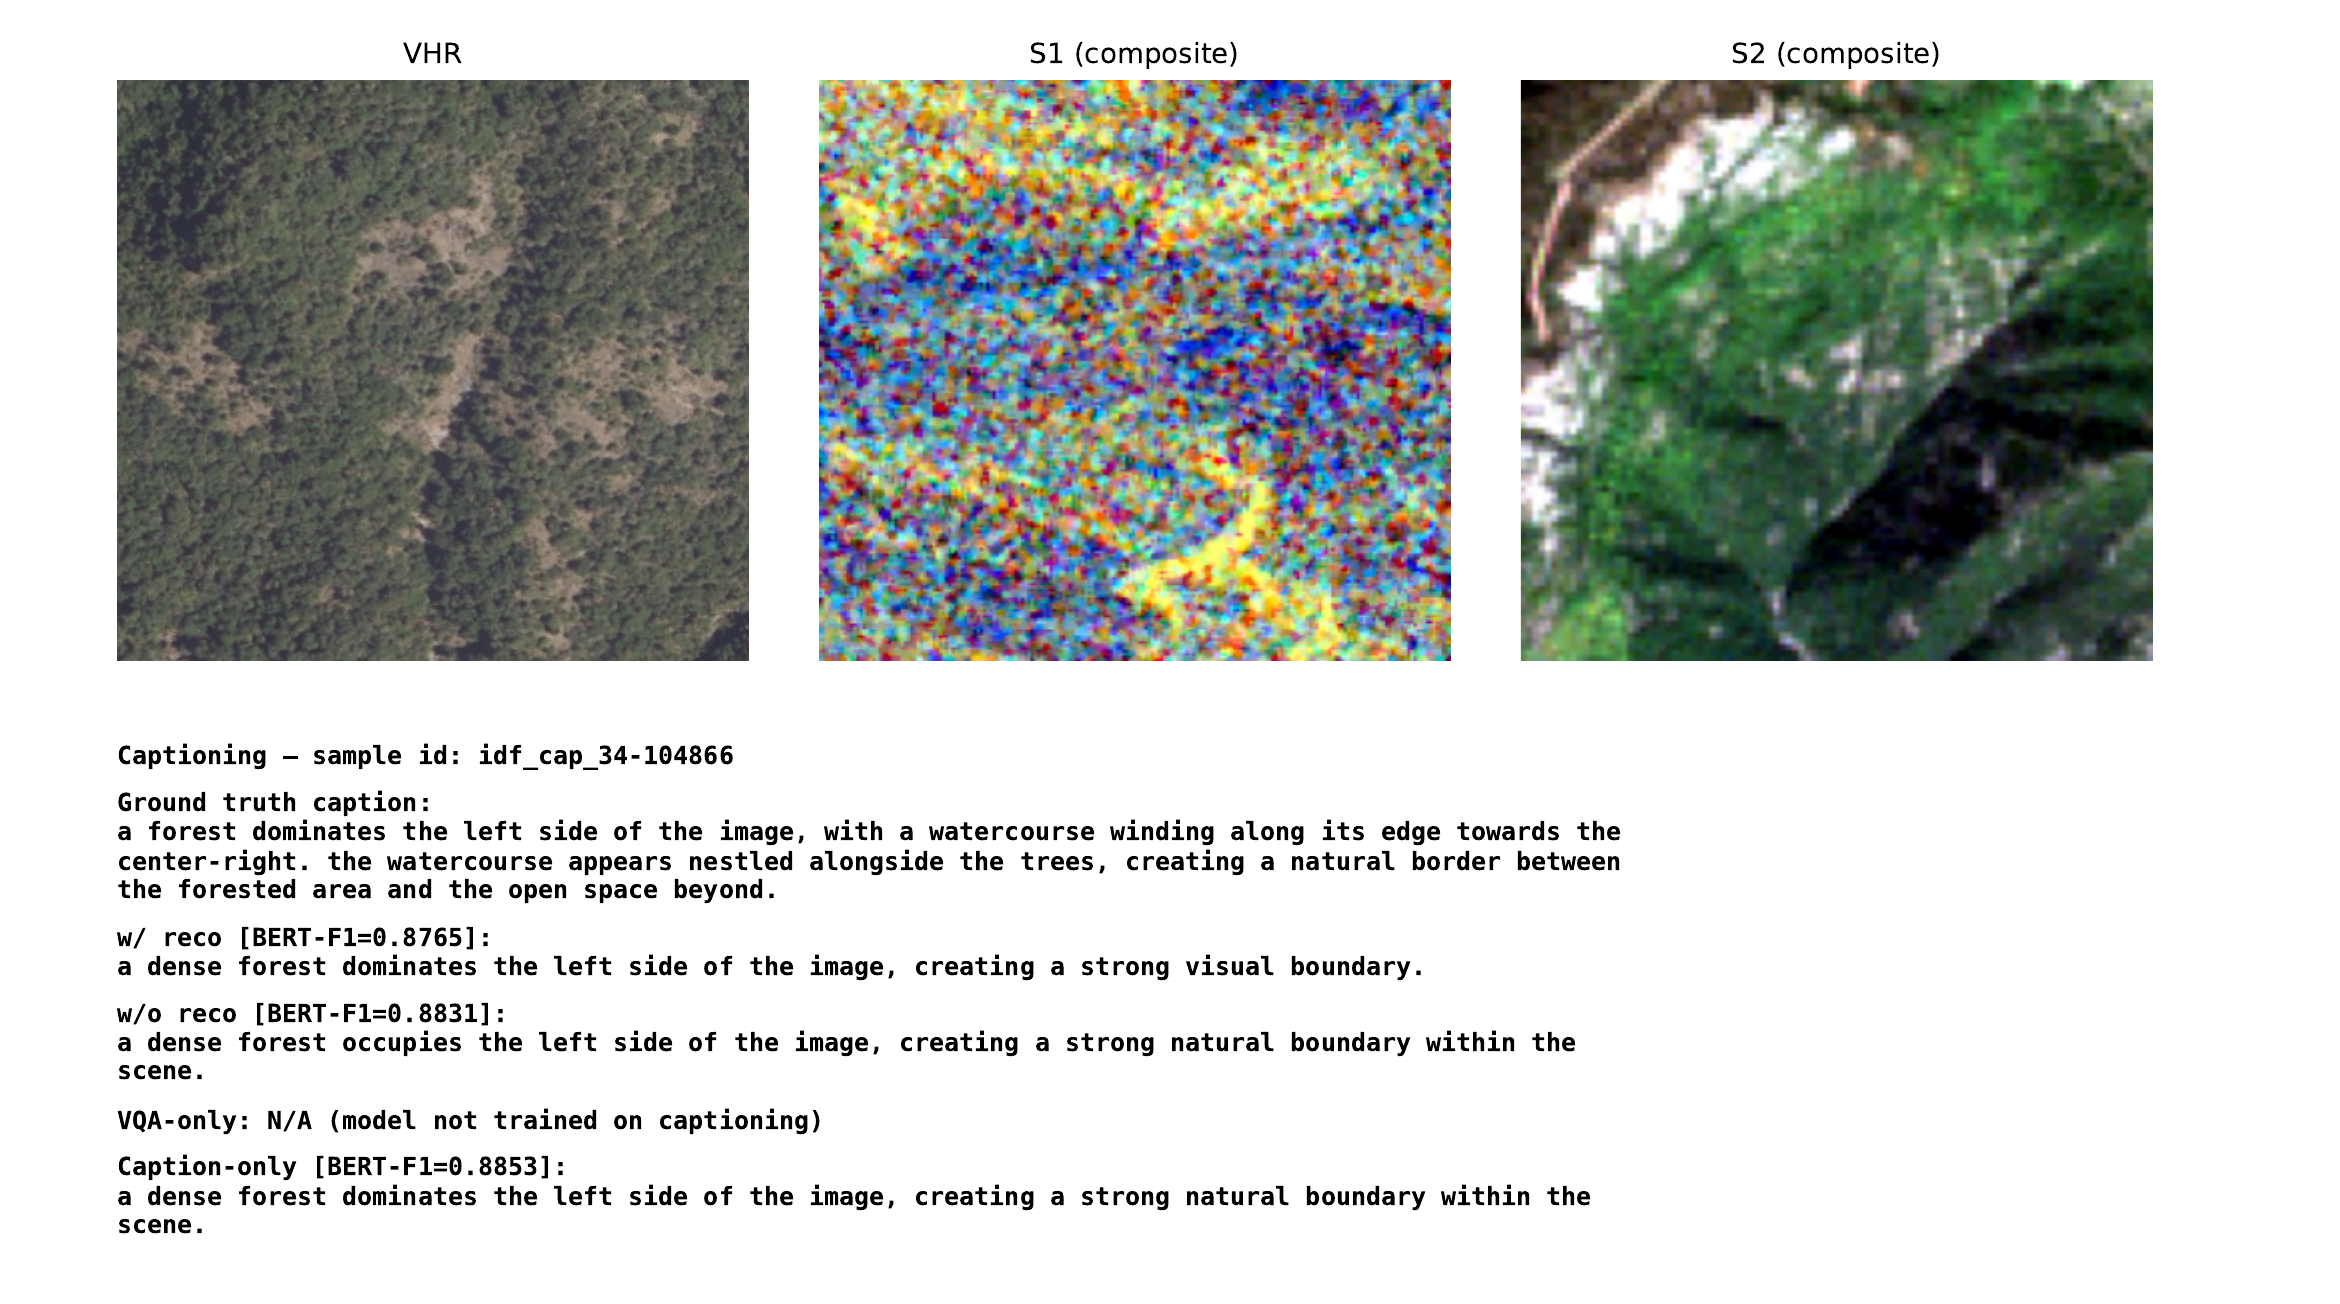
\includegraphics[width=0.85\textwidth]{images/multitask/qual_captioning.png}
\caption{Generated captions from each captioning-capable configuration
for the same VHR/SAR/multispectral triplet, alongside the ground-truth caption and
each configuration's BERTScore F1.}
\label{fig:chap6_qual_caption}
\end{figure}

In the example of Figure~\ref{fig:chap6_qual_caption} all three configurations correctly identify the dominant forest and
describe it as forming a boundary, but none mentions the watercourse
that the ground-truth caption explicitly describes as running along
the forest's edge, despite each scoring above 0.87 BERTScore F1. This
illustrates a limitation of embedding-based similarity metrics
discussed in Section~\ref{sec:chap6_setup}: a caption can omit a
salient detail entirely and still score highly if the retained content
is semantically close to the reference. The three configurations are,
by this metric, nearly indistinguishable on this example, despite
omitting the same real piece of information.

\begin{figure}[ht]
\centering
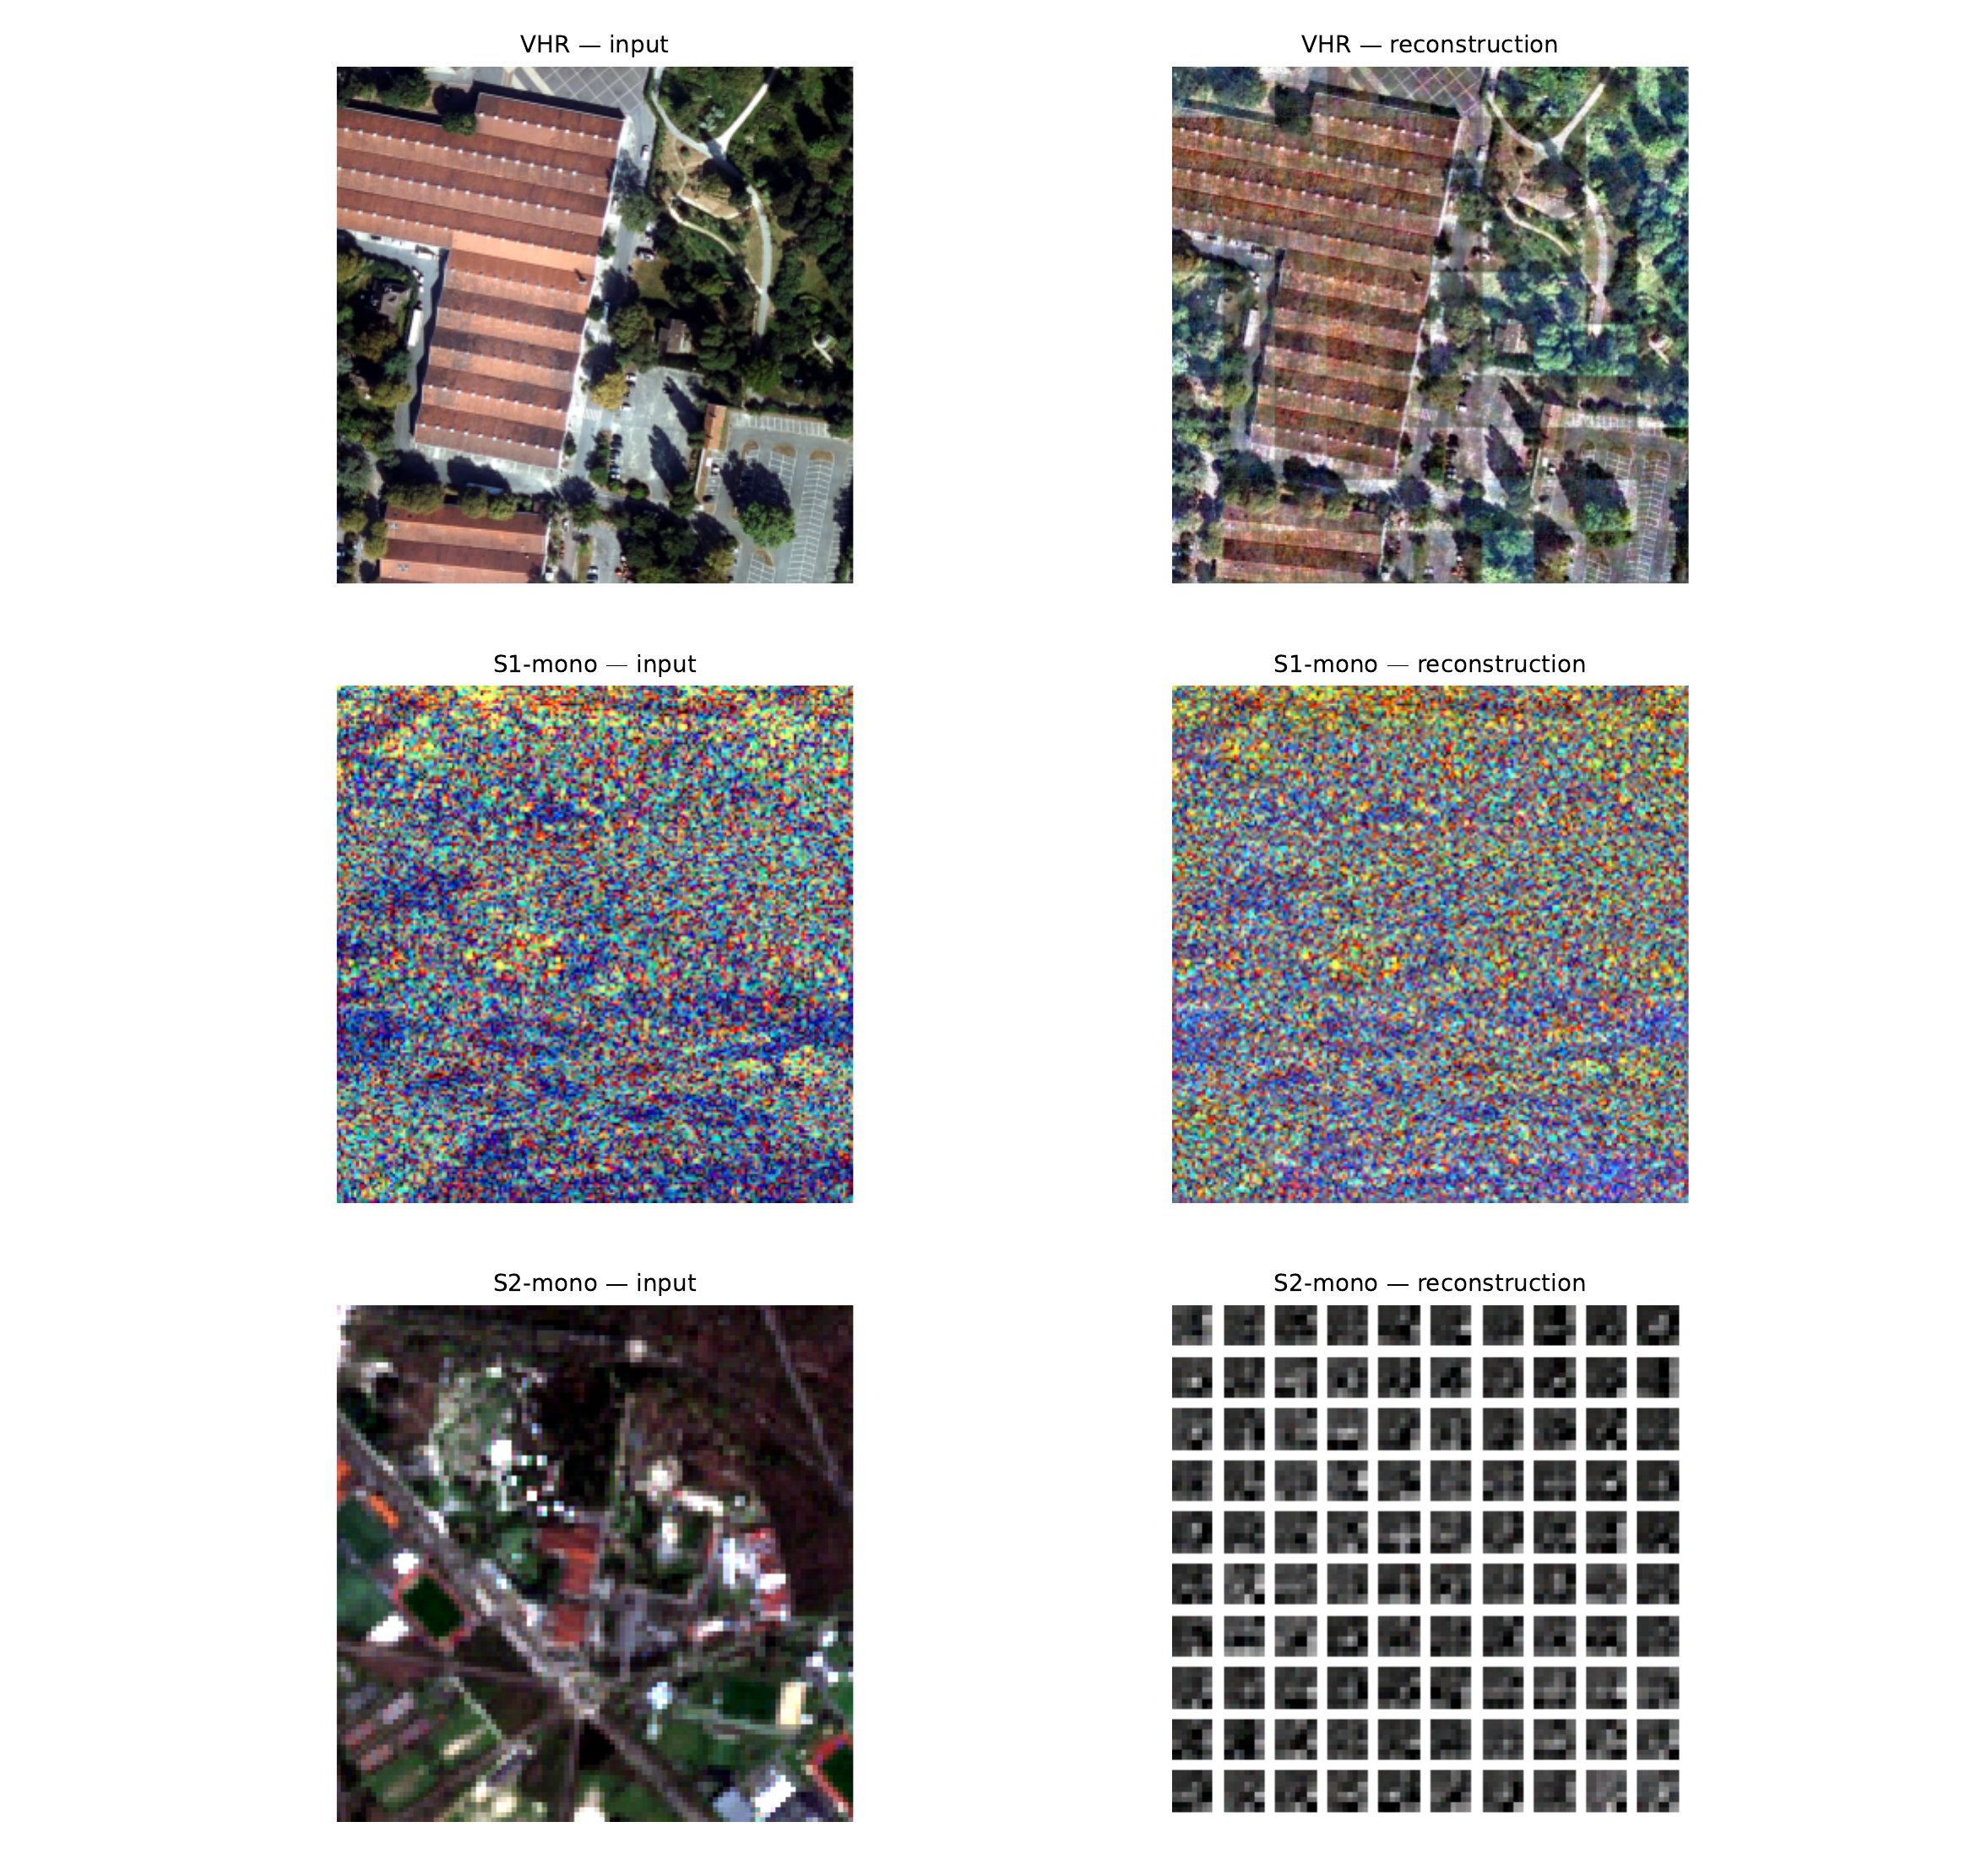
\includegraphics[width=0.85\textwidth]{images/multitask/qual_reconstruction.png}
\caption{Input and reconstructed patches for the VHR, SAR, and
multispectral modalities of a single TAMMI sample.}
\label{fig:chap6_qual_reco}
\end{figure}

In Figure~\ref{fig:chap6_qual_reco}, the VHR reconstruction recovers recognizable structure (building
outlines, road layout) closely matching the input; the SAR
reconstruction reproduces plausible speckle statistics, though a
pixel-level ground-truth comparison is not visually meaningful for
SAR. The multispectral reconstruction, however, shows a consistent,
spatially localized region of degraded content within each individual
patch, in the same relative position across patches and samples
regardless of the patch's actual content, unlike the ground truth's
dark regions, which vary in position with scene content as expected.
Isolating individual, unstitched patches traced this pattern to the
level of a single patch, ruling out stitching order and display-side
stretching as causes. It is consistent with information loss from
unpooling operations' max-pooling indices being systematically biased
at the very small ($10\times10$) patch resolution used for this
modality, though confirming this would require further architectural
investigation beyond the scope of this study.

\subsection{Discussion}
\label{sec:chap6_discussion}

Taken together, these results echo the RS-LLaVA finding already
discussed in Section~\ref{sec:rw-captioning-challenges}: single-task
training matches or exceeds multi-task training on both tasks studied
here, and reconstruction specifically does not measurably help
captioning. This is consistent with, rather than contradicting, this
chapter's framing: the premise motivating datasets and models that
combine these tasks is that joint training helps, and the aggregate
metrics above do not support that premise for either task. Combined
with the RS-LLaVA result, this provides a second, independent
measurement, on a different dataset, architecture, and task
combination, of the same pattern: assumed multi-task synergy in RS
vision-language models does not straightforwardly hold once measured
directly.

The reconstruction finding (Figure~\ref{fig:chap6_qual_reco}) offers a
partial, modality-specific explanation for this. Since
$\mathcal{L}_\text{rec}$ sums over all three visual modalities jointly
(Section~\ref{sec:chap6_method_reconstruction}), a modality-specific
weakness in the multispectral reconstruction would dilute the
aggregate reconstruction signal without being visible in the aggregate
loss value alone, plausibly contributing to why enabling reconstruction
("w/ reco") did not translate into a measurable downstream benefit for
either task.

At the same time, this chapter's aggregate metrics do not, on their
own, rule out category-specific synergy: the flooding-question example
(Figure~\ref{fig:chap6_qual_vqa_success}) shows the full multi-task
model succeeding where the single-task baseline fails. A per-question-type breakdown,
analogous to the one reported for MM-RSVQA in
Chapter~\ref{chap:tammi} and for the augmentation study in
Chapter~\ref{chap:llm_augmentation}, would clarify whether this
reflects a genuine category-specific effect or an isolated case, and
is a natural extension of this study, discussed further in
Section~\ref{sec:chap6_conclusion}.

\section{Conclusion and Limitations}
\label{sec:chap6_conclusion}

This chapter extended TAMMI with captions and introduced a unified
architecture combining cross-modal contrastive alignment, reconstruction,
and a shared generative decoder for captioning and VQA, then used it to
study, rather than assume, whether reconstruction and joint
captioning-VQA training improve performance on either task. At the
level of aggregate metrics, neither does: single-task training matches
or outperforms every multi-task configuration on both captioning and
VQA. This adds a second data point, alongside RS-LLaVA
(Section~\ref{sec:rw-captioning-challenges}), to the pattern that assumed
multi-task synergy in RS vision-language models does not straightforwardly
hold when measured directly.

\textbf{Limitations.} This study is conducted at the level of aggregate
metrics; a per-question-type breakdown, analogous to the one reported
for MM-RSVQA in Chapter~\ref{chap:tammi} and for the augmentation study
in Chapter~\ref{chap:llm_augmentation}, would clarify whether the
absence of synergy found here holds uniformly across question types or
masks category-specific effects, and is left for future work. Beyond
this, the study is conducted on a single dataset (TAMMI) and a single
architecture; whether the same pattern holds for other RS multi-task
combinations, or for architectures where reconstruction and generation
share more capacity than in the fusion design used here, remains open.
Finally, the multispectral reconstruction weakness identified in
Section~\ref{sec:chap6_discussion} was investigated only to the point
of localizing it, confirming the specific
mechanism, and addressing it, most plausibly by replacing the 
multispectral decoder's index-based upsampling with a learned upsampling stage, 
would require retraining and is left for future work.